\subsection{Separately continuous bilinear mappings}

Let E, F, G be three locally convex spaces. For every bilinear mapping u from \(E \times F\) into G, and for every \(x \in E\) (resp. \(y \in F\) ), we denote by \(u(x, .)\) (resp. \(u(., y)\) ) the mapping \(y \mapsto u(x, y)\) (resp. \(x \mapsto u(x, y)\) ) from F into G (resp. from E into G).

DEFINITION 1. --- A bilinear mapping u from E × F into G is said to be separately continuous if, for all x ∈ E, the linear mapping u(x, .) from F into G is continuous, and for all y ∈ F, the linear mapping u(., y) from E into G is continuous.

The following proposition follows immediately from the definition.

PROPOSITION 1. --- For a bilinear mapping u from E × F into G to be separately continuous, it is necessary and sufficient that for all y ∈ F, the linear mapping u(., y) from E into G is continuous and that the linear mapping y ↦ u(., y) from F into \(\mathcal{L}_s(E; G)\) is continuous.

We can also say that, to every linear mapping \(v \in \mathcal{L}\left(\mathrm{F}; \mathcal{L}_{s}(\mathrm{E}; \mathrm{G})\right)\) is associated the bilinear mapping \((x, y) \mapsto v(y)(x)\) , then we define a linear bijection from \(\mathcal{L}(\mathrm{F}; \mathcal{L}_{s}(\mathrm{E}; \mathrm{G}))\) onto the vector space of separately continuous bilinear mappings from \(E \times F\) into G.

A separately continuous bilinear mapping from \(E \times F\) into G need not necessarily be continuous on \(E \times F\) (III, p.~47, exerc. 2; cf.~however III, p.~30, and IV, p.~26, th. 2).

The notion of a separately continuous bilinear form on a product \(E_{1} \times E_{2}\) of two locally convex spaces is directly related to that of a continuous linear mapping when \(E_{1}\) and \(E_{2}\) are assigned the weak topologies (II, p.~42), Suppose that \((\mathrm{E}_{1}, \mathrm{F}_{1})\) and \((\mathrm{E}_{2}, \mathrm{F}_{2})\) are two pairs of real (resp. complex) vector spaces in separating duality (loc. cit.); we assign to \(E_{i}\) (resp. \(F_{i}\) ) the weak topology \(\sigma(\mathrm{E}_{i}, \mathrm{F}_{i})\) (resp. \(\sigma(\mathrm{F}_{i}, \mathrm{E}_{i})\) ) for i = 1, 2, and denote by \(\mathrm{B}(\mathrm{E}_{1}, \mathrm{E}_{2})\) the vector space of separately continuous bilinear forms on \(E_{1} \times E_{2}\) . Applying prop. 1 to the case when G = K, we see that, for every bilinear form \(\Phi \in \mathrm{B}(\mathrm{E}_{1}, \mathrm{E}_{2})\) and every \(x_{2} \in E_{2}\) , the mapping \(x_{1} \mapsto \Phi(x_{1}, x_{2})\) is a continuous linear form on \(E_{1}\) , hence (II, p.~43, prop. 3) there exists one element, and only one \(^{d}\Phi(x_{2}) \in F_{1}\) such that

\[
\Phi (x _ {1}, x _ {2}) = \langle x _ {1}, ^ {d} \Phi (x _ {2}) \rangle\tag{1}
\]

for every \(x_1 \in \mathbf{E}_1\) and \(x_2 \in \mathbf{E}_2\) ; moreover, the mapping \(^d\Phi: \mathbf{E}_2 \to \mathbf{F}_1\) is linear and continuous for the (weak) topologies of \(\mathbf{E}_2\) and of \(\mathbf{F}_1\) .

Conversely, for every continuous linear mapping \(u: \mathrm{E}_2 \to \mathrm{F}_1\) the mapping \((x_1, x_2) \mapsto \Phi(x_1, x_2) = \langle x_1, u(x_2) \rangle\) is a separately continuous bilinear form on \(\mathrm{E}_1 \times \mathrm{E}_2\) , and we have \(u = {}^d\Phi\) . Thus we have defined an isomorphism \(d: \Phi \mapsto {}^d\Phi\) from \(\mathrm{B}(\mathrm{E}_1, \mathrm{E}_2)\) onto \(\mathcal{L}(\mathrm{E}_2; \mathrm{F}_1)\) , said to be canonical. Similarly the formula

\[
\Phi (x _ {1}, x _ {2}) = \langle {} ^ {s} \Phi (x _ {1}), x _ {2} \rangle\tag{2}
\]

defines a canonical isomorphism \(s: \Phi \to {}^s\Phi\) from \(\mathbf{B}(\mathbf{E}_1, \mathbf{E}_2)\) onto \(\mathcal{L}(\mathbf{E}_1, \mathbf{F}_2)\) ; we have evidently the commutative diagram

\begin{enumerate}
\def\labelenumi{(\arabic{enumi})}
\setcounter{enumi}{2}
\tightlist
\item
\end{enumerate}

\pandocbounded{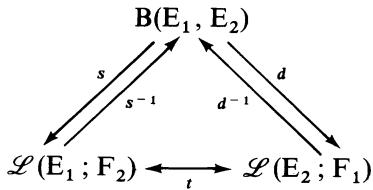
\includegraphics[keepaspectratio]{images/part001_08254dbd.jpg}}

where t is the isomorphism of transposition (II, p.~46, prop. 5 and corollary). In view of the definition of weak topologies on \(F_{1}\) and \(F_{2}\) , it is immediate that when \(\mathbf{B}(\mathbf{E}_{1}, \mathbf{E}_{2})\) , \(\mathcal{L}(\mathbf{E}_{1}; \mathbf{E}_{2})\) and \(\mathcal{L}(\mathbf{E}_{2}; \mathbf{F}_{1})\) are assigned the topology of simple convergence, the isomorphisms of diagram (3) are topological vector space isomorphisms.

